\chapter{The use of novel and alternative circuits' realization schemes as a way of power loss reduction}\label{lhrh}
%\chaptermark{test}


\indent In this Chapter the use of novel and alternative realization schemes of circuits as a way of power loss minimization is studied. The realization of filters exploiting the periodic structures approach in which the filter is composed of identical, electrically small unit cells is considered. The proposed approach allows for obtaining very compact and high-performance circuits which in turn leads to power loss minimization. Moreover, further power loss reduction can be obtained by unit cell`s topology optimization and an appropriate selection of the realization technique. This is due the total loss is a product of total length of the wave's propagation path and the attenuation constant, therefore can be reduced by reduction of one or both factors.
\\
\indent Filters are one of the basic building blocks of any communication system. Analysis and design of such components are subjects of extensive studies of scientific and industrial communities resulting in many different approaches and realizations being proposed. Among others, the periodic structures approach \cite{pozar} is very attractive allowing to reduce filter's design to a design of a single unit cell (UC) which exhibits the desired frequency response. The order of such a filter is dependent on the number $n$ of cascaded identical unit cells, where a single unit cell is an electrically small structure. Usually, unit cells featuring right-handed (RH) character, which is a property of conventional materials, are designed and used. However, the left-handed (LH) medium has gained in recent years a significant interest and poses an attractive alternative to RH materials due to it`s unique properties, not available in a conventional medium \cite{mm_lai}, \cite{caloz}. Although, in nature there are no homogeneous materials having left-handed properties, the effectively homogenous metamaterial transmission lines composed of a finite number of elementary unit cells featuring a left-handed character in microwave frequency range have been a subject of extensive research resulting in various realizations being proposed. On top of the interesting phase properties of such artificial transmission lines, their amplitude response and construction makes them well suitable for realization of microwave filters. Properly constructed topology of such unit cells supported with the design methodology allows to provide all kinds of frequency selective responses such as narrow- and wideband, bandpass and bandstop. 
\\
\indent The Author has proposed and developed various novel left-handed metamaterial-inspired unit cells, constructed of mostly or solely coupled and uncoupled transmission line sections, exhibiting all kinds of frequency selective response. The results of the conducted research have been a subject of three journal papers  published in \textit{IEEE Transactions on Microwave Theory and Techniqes}, \textit{IEEE Microwave and Wireless Components Letters} and \textit{International Journal of Electromagnetic Waves and Applications} as well as two conference papers presented at \textit{Mediterranean Microwave Symposium (MMS`17)} and accepted for \textit{International Conference on Microwave, Radar and Wireless Communications (MIKON`18)}, both under the auspices of \textit{Institute of Electrical and Electronics Engineers}, which constitute the Chapter.
\\
\indent In Section \ref{tmtt_lh}, a novel metamaterial structures featuring left-handed and composite right/left-handed (CRLH) characters are presented. The proposed unit cells utilize sections of coupled transmission lines. It is shown that by taking advantage of the coupling between transmission lines an additional degree of freedom is achieved, and therefore, the design process of artificial transmission lines is more flexible. The general behavior of each of the proposed circuits is presented and analyzed. Moreover, the design equations are formulated and the design process of each unit cell is described. The usefulness and validity of the proposed unit cells are illustrated and verified by the design and measurements of compact artificial transmission line sections utilizing the presented structures. Moreover, possible applications toward bandpass filters` realization are discussed.
\\
\indent Following, in Section \ref{mwcl_dlh}, an innovative approach for realization of artificial transmission lines featuring a dual-composite right/left-handed character is presented. The circuits utilize a novel semi-distributed unit cell which is composed of sections of conventional transmission lines and a lumped capacitor. Such an approach allows for efficient modeling and convenient translation of model parameters (characteristic impedance and electrical length of transmission lines) into physical realization. Moreover, a single-layer microstrip realization is possible, making the unit cell attractive in practical applications. The proposed concept was experimentally verified by the design and measurements of an exemplary transmission line section and discussed in a context of possible applications in bandstop filters.
\\
\indent Moreover, in Section \ref{jewa_semi-distr}, the design of high-selectivity, pseudo-highpass filters is presented. The proposed circuits utilize a novel semi-distributed-element composite right-left handed unit cell composed of sections of transmission lines and a lumped capacitor. By proper balancing the structure, a very broad operation band can be obtained. Moreover, a single-layer microstrip realization is possible making the unit cell well suitable for low-cost filter realization. The proposed concept was experimentally verified by the design and measurements of an exemplary pseudo-highpass filter.
\\
\indent Additionally, in Section \ref{mms_semi-distr}, a realization of low-loss wideband bandpass filters utilizing a periodic structure approach is presented. The recently developed novel semi-distributed composite right-left handed unit cell is considered and adopted for the design of the proposed filters. It is shown that an appropriate balancing of the structure, i.e. the  selection of circuits` parameters allows for achieving very broad passband. Moreover, a suspended microstrip technique is utilized to reduce total insertion loss of the circuit. The presented approach has been confirmed by the realization of an exemplary low-loss wideband bandpass filter. Measured operation band is within 1.0 – 9.4 GHz with total loss ranging between 0.35 to 1.8 dB. The obtained results proved the applicability of the presented approach.
\\
\indent Finally, in Section \ref{mikon_distr}, a novel wideband band-pass unit cell is presented, used for the realization of a wideband pseudo-highpass filter employing the periodic structures approach. Low losses and circuit properties' control are obtained by the realization of the unit cell using solely distributed elements, i.e., transmission line stubs and a coupled-line section as well as the utilization of suspended stripline technique for circuit realization. Theoretical analysis of the unit cell as well as experimental results have been provided. An exemplary manufactured compact low-loss four-unit-cell filter features 1 - 9 GHz fundamental passband with very sharp lower roll-off and minimal insertion losses of 0.24 dB. The obtained results confirmed the performance of the proposed approach.

\cleardoublepage

\includepdf[pages=-,addtotoc={1,section,1,Right/left-handed transmission lines based on coupled transmission line sections and their application towards bandpass filters,tmtt_lh}, pagecommand={}, scale=.98]{chapter_3/tmtt_lh.pdf}

\cleardoublepage

%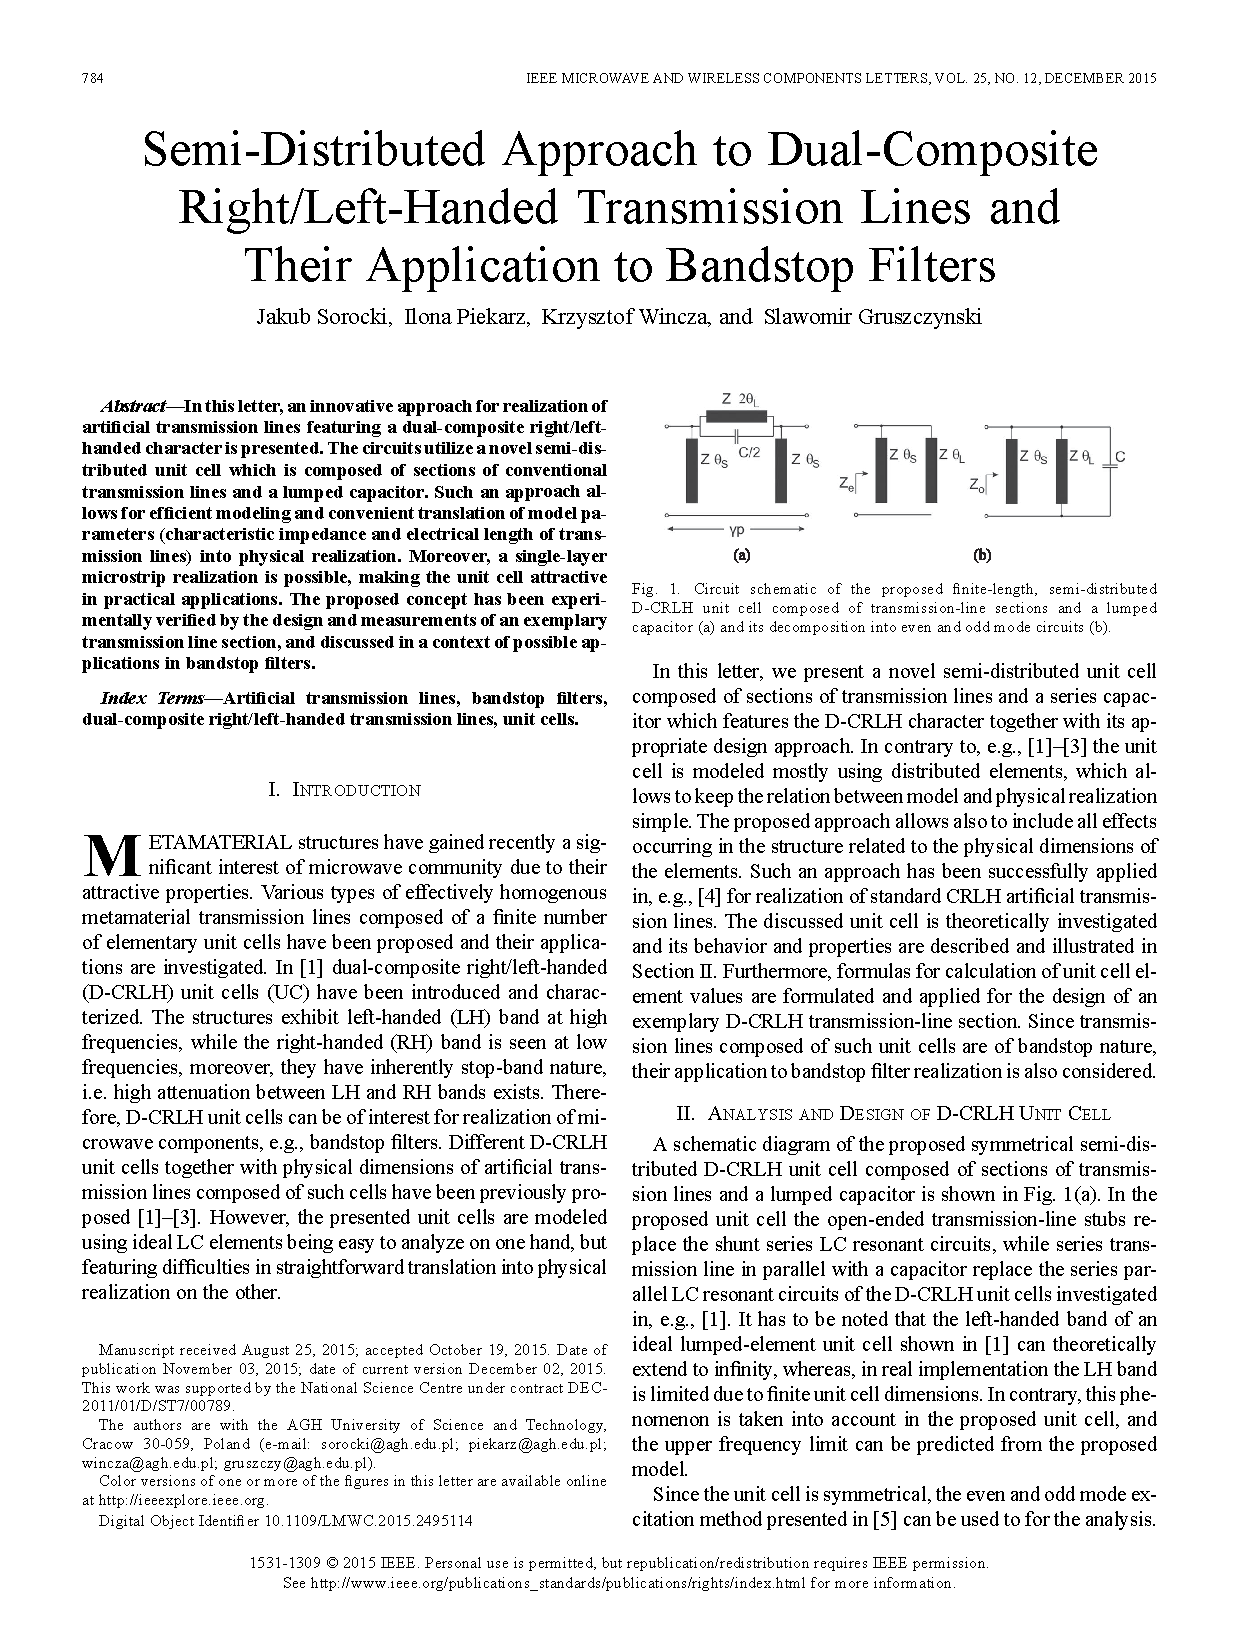
\includepdf[pages=-,addtotoc={1,section,1,Semi-distributed approach to dual-composite right/left-handed transmission lines and their application to bandstop filters,mwcl_dlh}, pagecommand={}noautoscale=true,offset=-30 30, frame, scale=.95, pagecommand={\sectionmark{test running title}}]{chapter_3/mwcl_dlh.pdf} , width=\textwidth
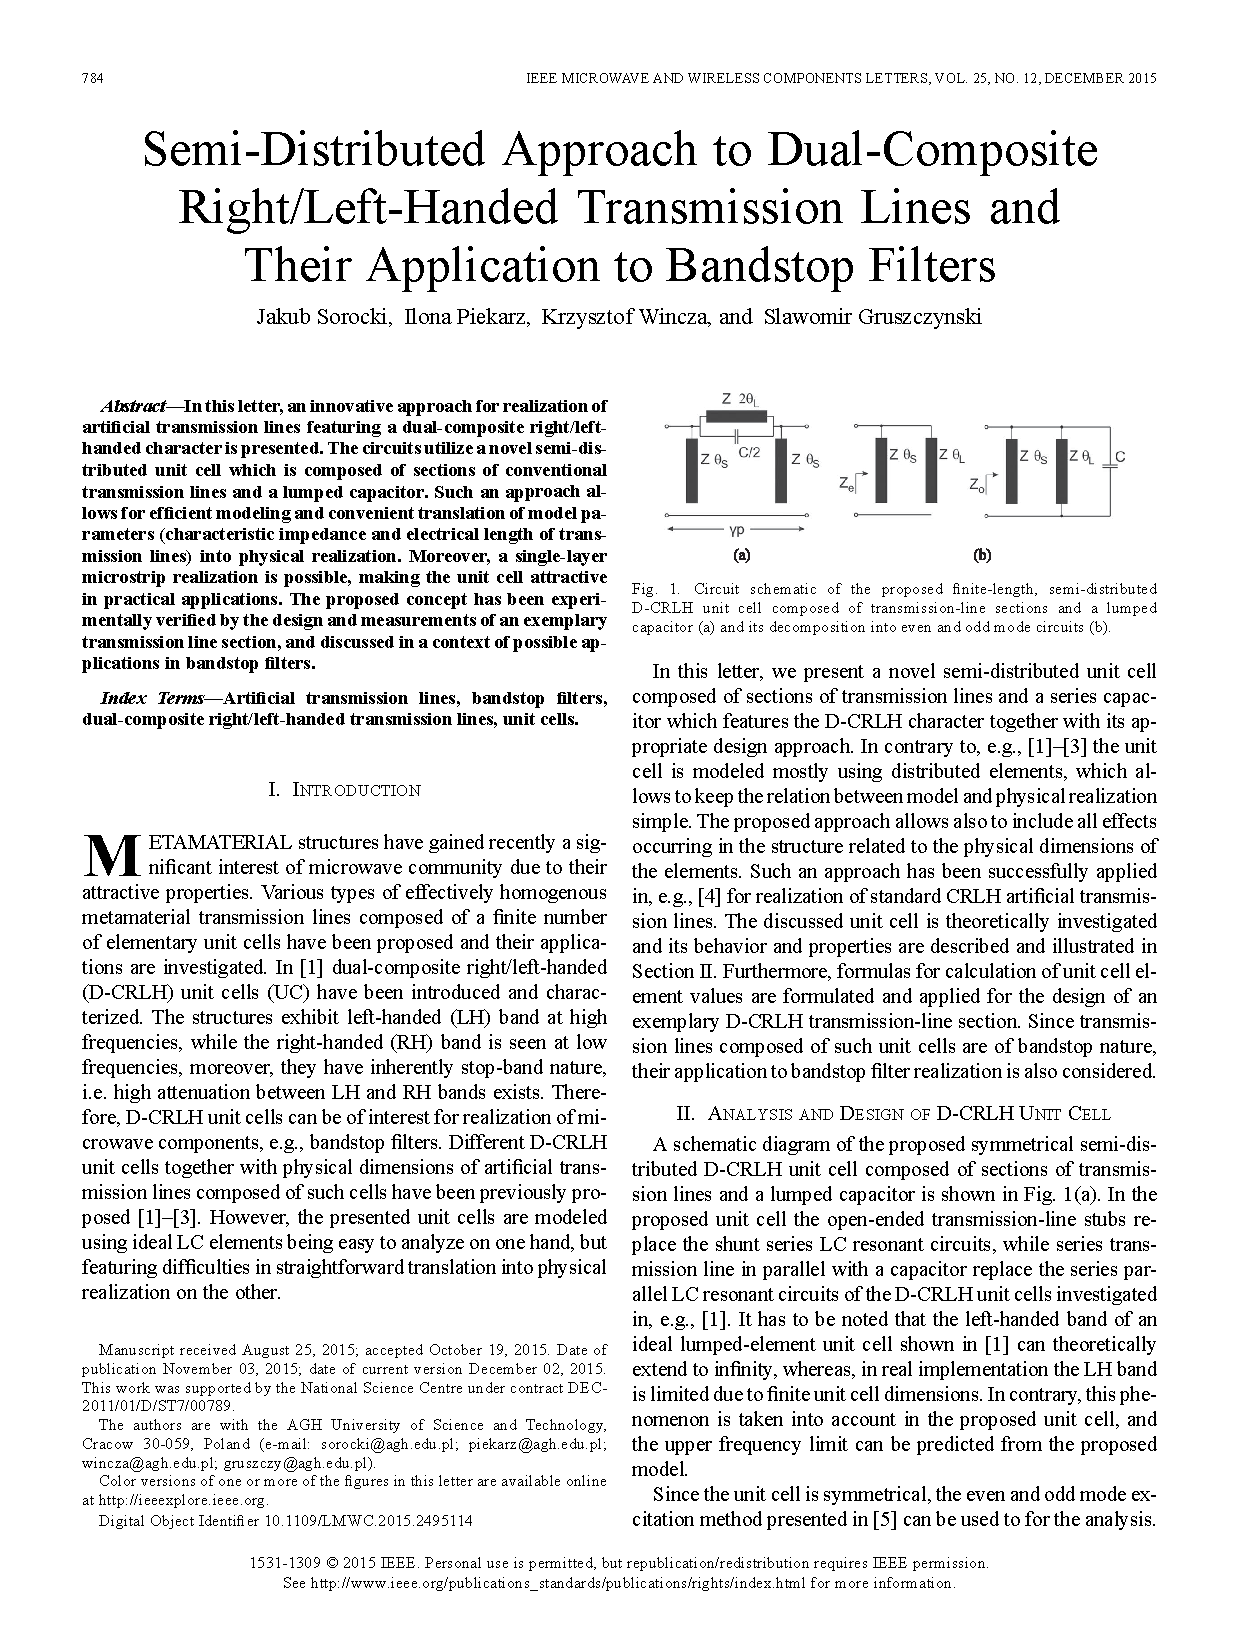
\includepdf[pages=-,addtotoc={1,section,1,Semi-distributed approach to dual-composite right/left-handed transmission lines and their application to bandstop filters,mwcl_dlh}, pagecommand={}, scale=.97]{chapter_3/mwcl_dlh.pdf}
\cleardoublepage

\includepdf[pages=-,addtotoc={1,section,1,Pseudo-highpass filters based on
semi-distributed balanced composite right/left-handed unit cells,jewa_semi-distr}, pagecommand={}, scale=.97]{chapter_3/jewa_semi-distr.pdf}

\cleardoublepage

\includepdf[pages=-,addtotoc={1,section,1,Low-loss wideband bandpass filters using
semi-distributed unit cells,mms_semi-distr}, pagecommand={}, scale=.97]{chapter_3/mms_semi-distr.pdf}

\cleardoublepage

\includepdf[pages=-,addtotoc={1,section,1,Low-loss pseudo-highpass filters using distributed-element unit cells,mikon_distr}, pagecommand={}, scale=.97]{chapter_3/mikon_distr.pdf}

\cleardoublepage